
\documentclass[letterpaper, portrait, margin=0.8in]{article}

\usepackage{geometry}
\usepackage{minted}
\usepackage{graphicx}
\newcommand{\HRule}{\rule{\linewidth}{0.5mm}}
\usepackage{wrapfig}
\usepackage{subcaption}
\usepackage{setspace}
\usepackage{booktabs}
\usepackage[T1]{fontenc}
\usepackage[font=small, labelfont=bf]{caption}
\usepackage[protrusion=true, expansion=true]{microtype}
\usepackage[english]{babel}
\usepackage{sectsty}
\usepackage{url, lipsum}   
\usepackage{tcolorbox}
\usepackage{lipsum}

\newenvironment{myexampleblock}[1]{%
    \tcolorbox[beamer,%
    noparskip,breakable,
    colback=LightGreen,colframe=DarkGreen,%
    colbacklower=LimeGreen!75!LightGreen,%
    title=#1]}%
    {\endtcolorbox}

\newenvironment{myalertblock}[1]{%
    \tcolorbox[beamer,%
    noparskip,breakable,
    colback=LightCoral,colframe=DarkRed,%
    colbacklower=Tomato!75!LightCoral,%
    title=#1]}%
    {\endtcolorbox}

\newenvironment{myblock}[1]{%
    \tcolorbox[beamer,%
    noparskip,breakable,
    colback=white,colframe=DarkBlue,%
    %colbacklower=DarkBlue!75!LightBlue,%
    title=#1]}%
    {\endtcolorbox}


\newenvironment{myitemize}
{ \begin{itemize}
    \setlength{\itemsep}{0pt}
    \setlength{\parskip}{0pt}
    \setlength{\parsep}{0pt}     }
{ \end{itemize}                  }









\begin{document}

\title{ \LARGE \normalsize {The International School of Trigger and Data Acquisition 2017} \vspace{10cm} \\
		\LARGE \textbf{\uppercase{System on Chip - FPGA}} \\ 
		\normalsize \today \vspace*{5\baselineskip}}

\date{}

\maketitle
\newpage
\tableofcontents
\newpage

%-------------------------------------------------------------------------------
% Section title formatting
\sectionfont{\scshape}
%-------------------------------------------------------------------------------

%-------------------------------------------------------------------------------
% BODY
%-------------------------------------------------------------------------------

\section{INTRODUCTION}

This laboratory will familiarize you with the \textbf{All Programmable System on Chip (AP SoC)} processor-centric platform which offers software, hardware and I/O programmability in one single chip.



{\color{red}To be added 2-3 paragraphs}

\newpage

\section{IMPLEMENTATION IN HARDWARE}

\subsection{Block diagram of the study case}


{\color{red} put picture FPGA \\ put picture block diagram}

We are going to introduce all the concepts of the block diagram throughout the next pages of the laboratory.


\newpage

\subsection{Getting started with the environment}

\textbf{Vivado Design Suite}, along with the \textbf{Xilinx Software Development Kit (XSDK)} are the main applications used in this laboratory. The first one will be mainly used for the hardware development(talking to the FPGA), while XSDK will be used for embedded C development (talking to the ARM processor). Vivado Design Suite has two important modes: \textit{project mode} and \textit{non-project mode}. In project mode, Vivado tool will automatically manage the design flow and directory structure. As you will become more advanced, the non-project mode will allow you to automatize your design flow using Tcl-language commands and scripts. 

\subsubsection{System on Chip Design Flow in Vivado Design Suite}

Vivado design flow is based on Advanced eXtensible Interface (AXI) standard protocol which provides great flexibility and customization for each of your applications. There are three important concepts related to the AXI interface that you need to know: the AXI Master, the AXI Interconnect and the AXI Slave. Their connectivity can be seen in the next diagram.


\begin{figure}[h!]
    \centering
    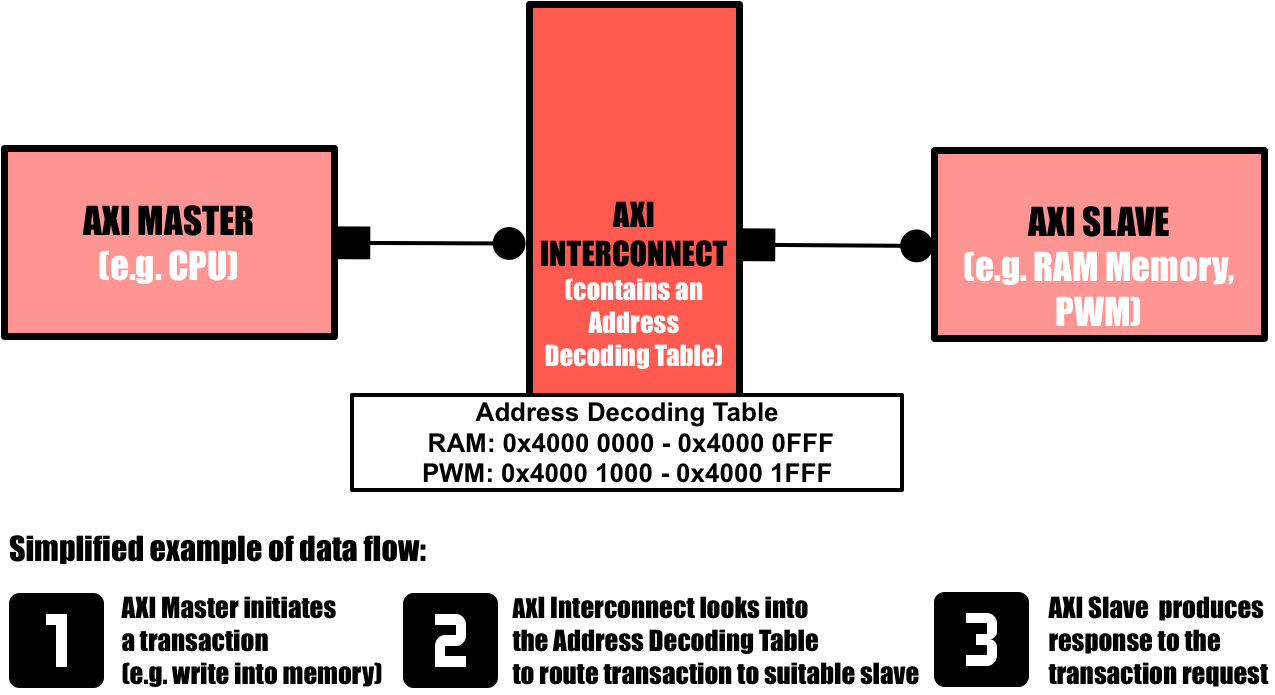
\includegraphics[width=0.9\textwidth]{img/AXI.png}
    \caption{AXI Architecture}
    \label{fig:axi}
\end{figure}

As we have talked about customization per application, you can use two types of advanced eXtensible interfaces (AXIs): AXI Stream and AXI Memory Mapped (MM). Basically, a simple application such as computation of some stream of data can make use of AXI Stream, while a more complex one (e.g. writing on a memory) might need access to addresses (so AXI MM comes in place). Their diagrams can be seen in Figure  \ref{fig:axi_mm_stream}. \textbf{In our case, we will use an AXI Memory Mapped architecture, and PWM (Pulse Width Modulation) slave module to control LEDs and a buzzer.}

\begin{figure}[h!]
    \centering
    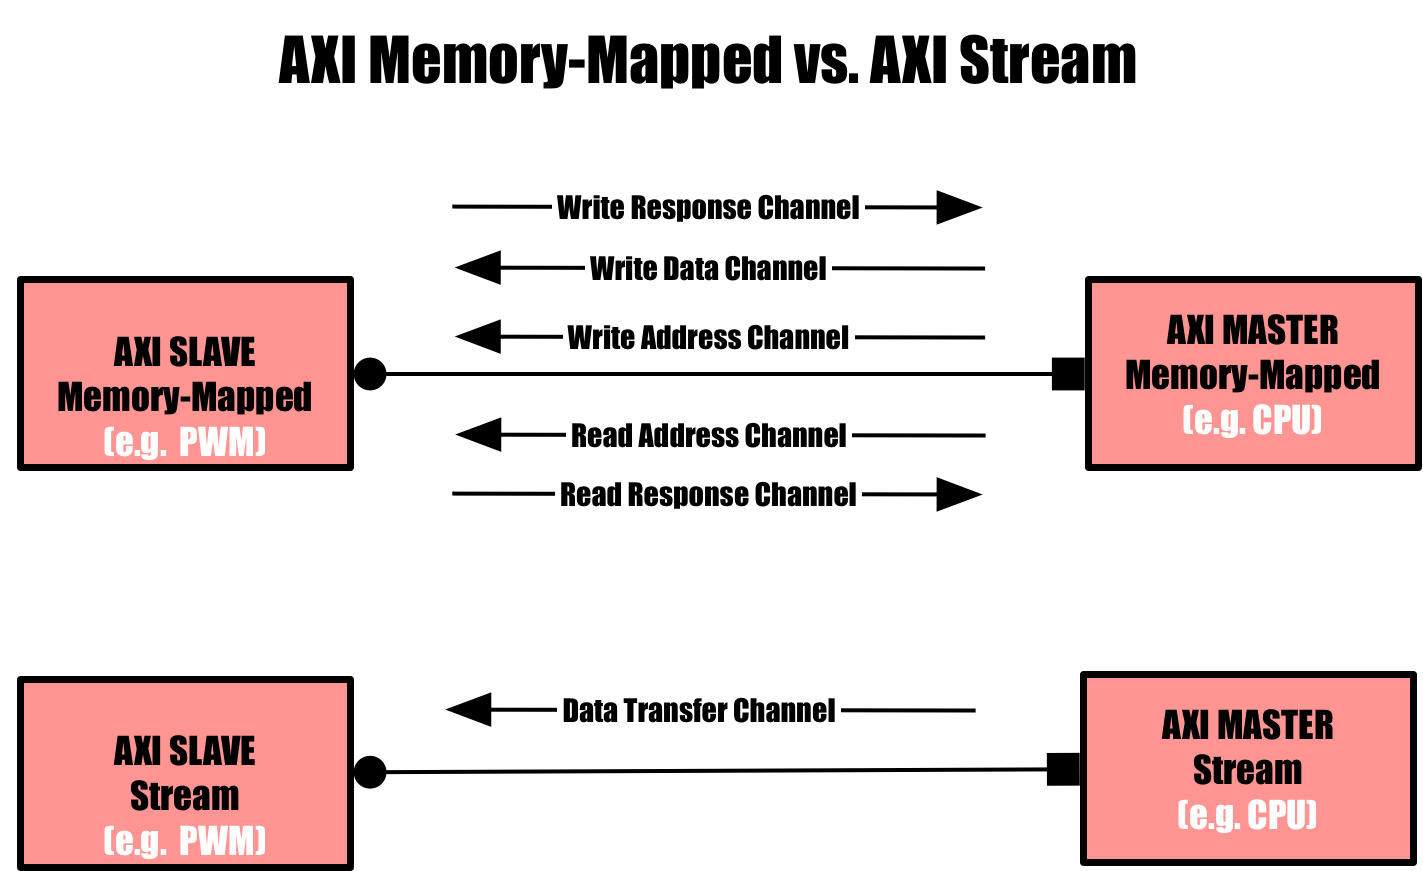
\includegraphics[width=0.6\textwidth]{img/axi_mm_stream.png}
    \caption{AXI Memory Mapped and AXI Stream arhitecture}
    \label{fig:axi_mm_stream}
\end{figure}

\newpage

\subsubsection{Pulse Width Modulation (PWM) Slave Peripheral}

\textbf{INTRODUCTION}

In Figure \ref{fig:pwm_waveform}, you can see a basic PWM waveform.  There are two important parameters that characterize the PWM waveform: \textbf{the duty cycle} and the \textbf{PWM period}. The PWM  period is set by "waiting/counting" a number of clock cycles,  while the duty cycle  tells us, in one period, how many clock cycles the PWM signal is low . 

\begin{figure}[h!]
    \centering
    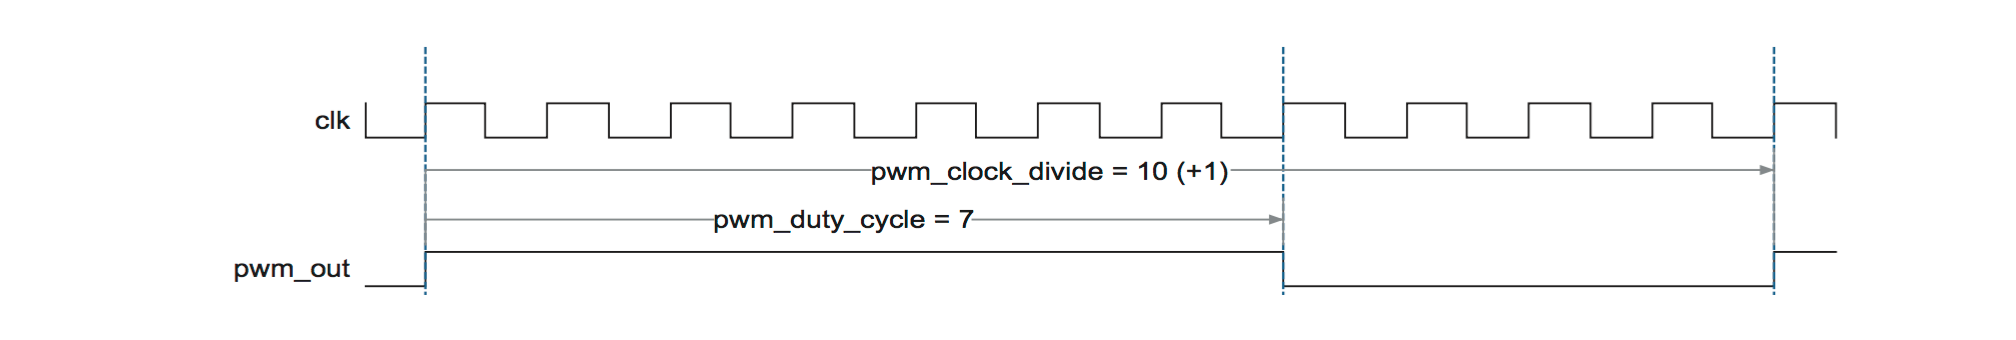
\includegraphics[width=\textwidth]{img/pwm_waveform.png}
    \caption{PWM waveform (Source: Application Note 333, Altera)}
    \label{fig:pwm_waveform}
\end{figure}

Now let's see how we are going to use these two simple parameters to make an RGB LED change its color and a buzzer "sing".
\begin{itemize}
\item \textbf{RGB LED}

In the case of RGB LED, we need 3 PWMs signals (one per each color), such that the brightness of each of the three LEDs can be controlled independently. 

\textbf{\textit{How do we choose the PWM period?}} The driving frequency of the PWM should be fast enough to avoid the flicker effect. A normal human being sees this effect until up to 100 to 150 Hz, so a higher frequency should be better to avoid this effect. For this exercise, we will use a frequency of 1.5 KHz.

\textbf{\textit{How do we choose the PWM duty cycle?}} The brightness of the LEDs is controlled by the duty cycle. This is up to you to do experiments. You can choose basically any duty cycle in the range of 0$\%$ to 100$\%$.

\item \textbf{BUZZER}

Previously, for the LED, we kept constant the frequency and varied the duty cycle. Now, for the buzzer, it will be the opposite: a constant duty cycle and a varying frequency.

The buzzer is based on the reverse of piezoelectricity which means that if you produce a voltage, the piezoelectric material from the buzzer gets distorted. When you stop producing that voltage, it gets back to its original shape. When producing this voltage fast enough (like in the PWM waveform), the buzzer will start to oscillate and "sing". This is the reason why we are currently controlling the frequency of PWM, and not the duty cycle. In this case, the duty cycle can be interpreted as the volume of the buzzer.

\textbf{\textit{How do we choose the PWM frequency?}}  The frequency range that the human ear is able to hear is between 20 Hz and 20.000Hz such as the PWM frequency for our buzzer will also fall in this range.


\textbf{\textit{How do we choose the PWM duty cycle?}} Maximum sound is achieved with a 50$\%$ duty cycle. In this exercise, we suggest a duty cycle of 10$\%$ such as you will not bother your neighbors when testing your application, but you are free to experiment with other values as well.
\end{itemize}


\textbf{PWM SLAVE LOGIC}

The PWM waveform can be generated either using the ARM processor and a Timer, or implemented on the FPGA. In this exercise, we will use this slave interface implemented in VHDL (VHSIC Hardware Description Language) language, directly on the fabric. 

In Figure \ref{fig:pwm_logic_block}, the block diagram of the slave peripheral is showed. The explanation of each output/input as well as the internal registers is presented in Table \ref{tab:reg_def}. Read it quickly now, but refer to it when you will start implementing the design. 

\begin{figure}[h!]
    \centering
    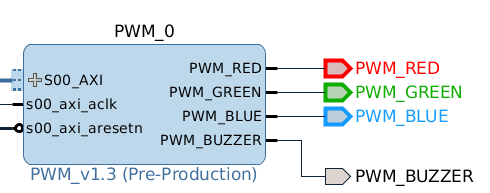
\includegraphics[width=0.7\textwidth]{img/pwm_logic_block.png}
    \caption{PWM Slave IP}
    \label{fig:pwm_logic_block}
\end{figure}


\begin{table}[h!]
\centering
\begin{tabular}{|p{6.3cm}|p{3cm}|p{7cm}|}
\hline
\textbf{Signal/register}                     & \textbf{Type}              & \textbf{Description}                                                                                                                       \\ \hline
PWM\_RED \newline  PWM\_BLUE \newline  PWM\_GREEN \newline  PWM\_BUZZER & std\_logic (1-bit)         & Signal set 1 or 0 to create the PWM waveform to control the LEDs and Buzzer                                                                \\ \hline
counter\_pwm                                 & integer (16-bit)           & Register that increments up to PWM\_LEDS\_PERIOD\_COUNTER in order to set the PWM period, and reset to 0 once its value equals that period \\ \hline
PWM\_LEDs\_PERIOD\_COUNTER                   & integer (16-bit)            & Parameter that can be set from the User Interface to choose the period of the PWM. This value is calculated using equation (1).            \\ \hline
counter\_pwm\_buzzer                         & integer(16-bit)            & Register similar to \textit\{counter\_pwm\}                                                                                                \\ \hline
slv\_reg0 \newline  slv\_reg1 \newline  slv\_reg2              & std\_logic\_vector (32-bit) & Local signals memory mapped to the address space, and used to set the duty cycle of the PWM waveform for red, blue and green color.        \\ \hline
slv\_reg3                                    & std\_logic\_vector (32-bit) & Local signal memory mapped to the address space, and used to set the PWM period of the PWM waveform for the buzzer                         \\ \hline


S00\_AXI & set of registers & This interface pin is connected to the AXI\_Interconnect which makes the link to the AXI Master, as explained conceptually above. \\ \hline

s00\_axi\_aclk & std\_logic (1-bit) & Synchronized the logic peripheral. Currently, it is connected to the Master Clock. \\ \hline

s00\_axi\_aresetn & std\_logic (1-bit) & Resets the peripheral. Connected to the reset of the Master reset which is mapped to the reset button on the Z-Turn board.\\ \hline

\end{tabular}
\caption{Register definition for the PWM Slave}
\label{tab:reg_def}
\end{table}


%\noindent\rule{18cm}{1pt}

\clearpage

\subsubsection{Implementation}

In order to start our implementation, the next steps should be followed:

\begin{enumerate}
\item Open an Ubuntu terminal and type 
\begin{minted}{c}
vivado &
\end{minted}

Vivado Design Suite is launched and a Getting Started Page is displayed.

\item Create a new project and set the project name to \textbf{Peripherals}. 

Select \textbf{Next} and tick \textbf{RTL Project}. 
Next, you will be asked to add sources to your design. For the moment, we will keep the project empty. However, we need to specify \textbf{VHDL} for both \textit{Target Language} and \textit{Simulator Language}. Press \textbf{Next}, and you will be asked about Existing IP and Constrains files. Keep them both empty again.

Now, we need to choose the platform where we implement our design. The development board is entitled MYS-7Z010-C-S Z-turn (Figure \ref{fig:board}).  Press \textbf{Next} and \textbf{Finish}.  Now, the project will initialize.
\begin{figure}[h!]
    \centering
    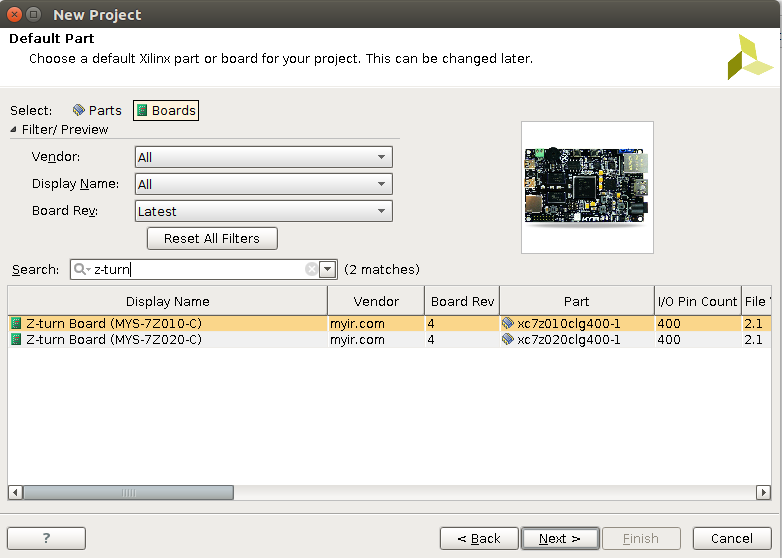
\includegraphics[width=0.85\textwidth]{img/board.png}
    \caption{Board Selection}
    \label{fig:board}
\end{figure}
 
\item  The \textbf{Peripherals} project should now look  similar to Figure \ref{fig:first_page}. In this project, we will implement the necessary files to control an RGB LED and a buzzer.

\begin{figure}[h!]
    \centering
    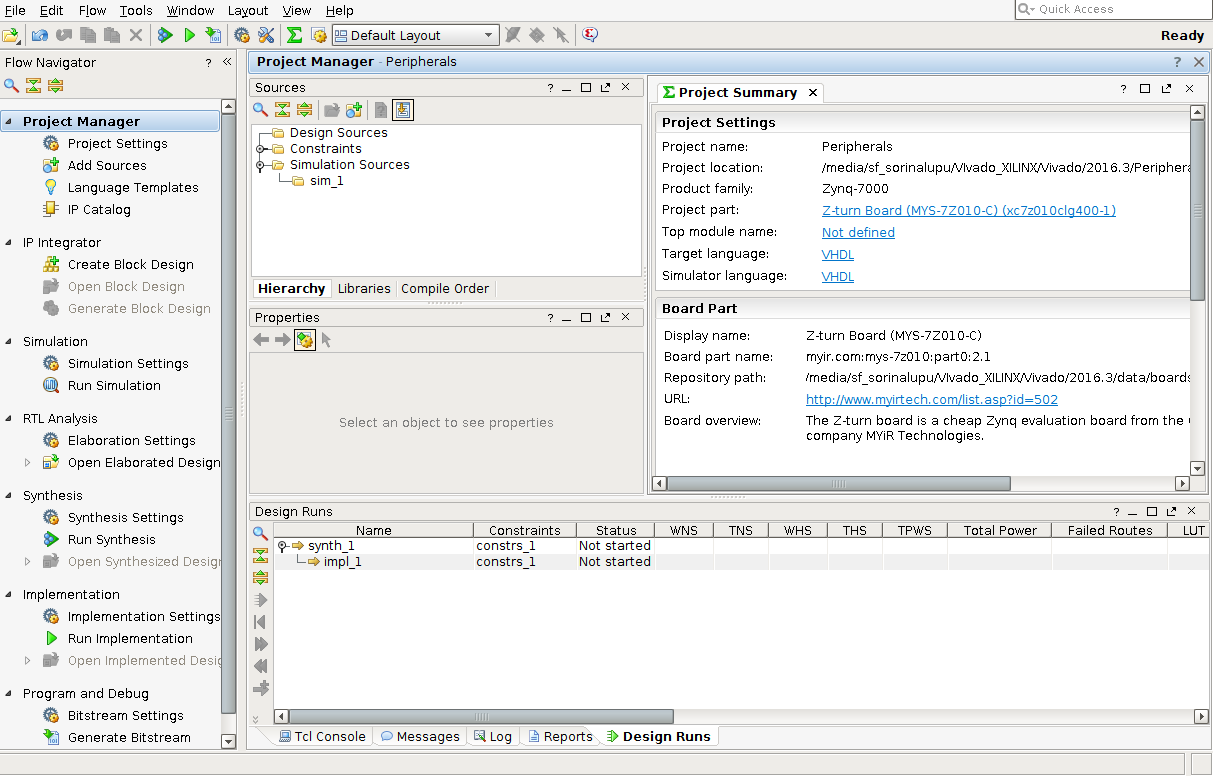
\includegraphics[width=0.85\textwidth]{img/project_first_page.png}
    \caption{Project Structure}
    \label{fig:first_page}
\end{figure}


\item Create the Block Design. On the left, in the Flow Navigator window, choose \textbf{Create Block Design} and call it \textbf{Peripherals}. Press OK, and now the environment should look like in Figure \ref{fig:diagram_second_page}. Vivado is based on an IP-centric design flow, in order to rapidly configure the AXI interconnect, AXI Masters and Slaves. 

\begin{figure}[h!]
    \centering
    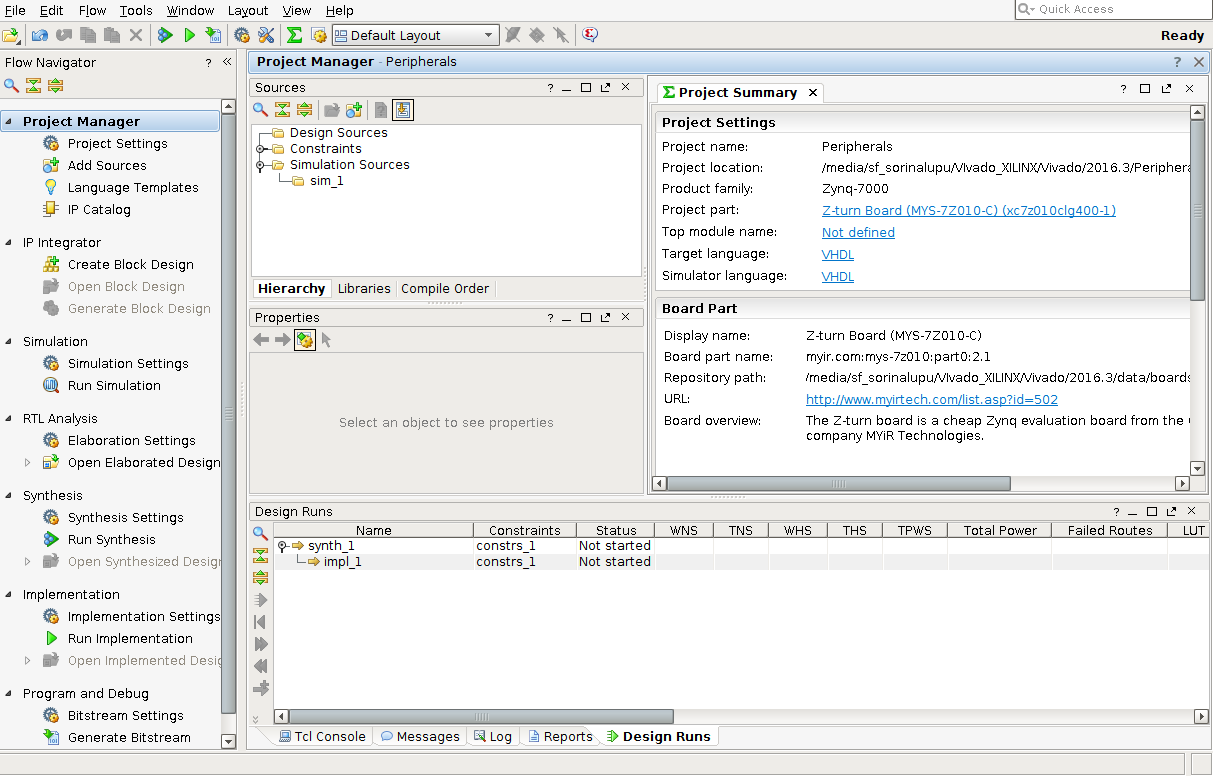
\includegraphics[width=0.85\textwidth]{img/project_first_page.png}
    \caption{Project Structure}
    \label{fig:diagram_second_page}
\end{figure}


\item Now we will add the AXI Master (Zynq7 Processing System) and the PWM IP (PWM\_v1.3) in the block diagram. The PWM IP was already implemented for you, such as you can choose it from the library, as in the pictures below. Press Add IP 
\includegraphics[width = 0.5cm]{img/icon_add.png}. 
 
 \begin{figure}[h!]
\centering
\begin{minipage}{.425\textwidth}
  \centering
  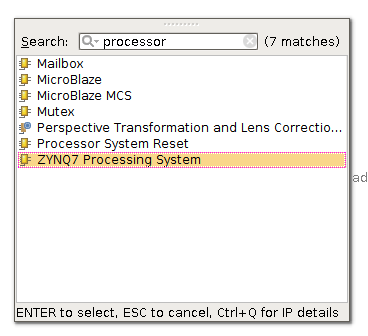
\includegraphics[width=0.8\linewidth]{img/diag_processor.png}
\end{minipage}%
\begin{minipage}{.425\textwidth}
  \centering
  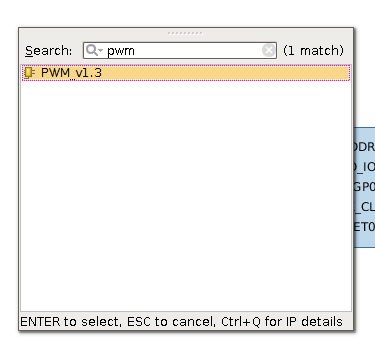
\includegraphics[width=0.8\linewidth]{img/diagram_pwm.png}
\end{minipage}
\caption{IP Blocks for Master and Slave}
\label{fig:diagram}
\end{figure}


Of course, there are other important IPs that should be added, such as AXI Interface or Processor System Reset, as well as the interconnectivity between them. However, the advantage of using Block Design is that these extra work is automated for you. 
Therefore, you should press {\color{blue}\underline{Run Block Automation}} and {\color{blue} \underline{Run Connection Automation}}, let the settings as default, press OK and let the Designer Assistance to do this work on your behalf. The window should now look similar to Figure \ref{fig:block_diagram_system}. However, the Design Assistant is placing the blocks in a not-very-organized way. For a better view, we advise you to click on the Regenerate Design button 
\includegraphics[width = 0.5cm]{img/icon_refresh.png} in the right Menu. Looks better, right?

\begin{figure}[h!]
    \centering
    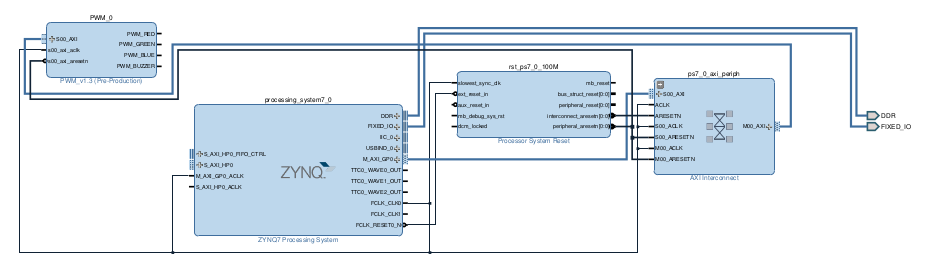
\includegraphics[width=0.85\textwidth]{img/block_automation_1.png}
    \caption{Block Diagram of our System}
    \label{fig:block_diagram_system}
\end{figure}


\item Let's dig into how the PWM Peripheral was designed in VHDL.

Right click on the PWM\_0 IP and select \textit{Edit in IP Packager}. Another project (Figure \ref{fig:ip}) will open that contains the files generated for this IP. Vivado Design Suite provides you with \textit{Packaging Steps} to configure the current IP. In the Source part, you will see an hierarchical design in VHDL. The top level is called \textit{PWM\_v1\_0.vhd} and contains an instantiation of the  \textit{PWM\_v1\_0\_S00\_AXI.vhd} where the logic is implemented. If you open  \textit{PWM\_v1\_0\_S00\_AXI.vhd}, you will see the registers specific to the AXI-Memory Map architecture (Figure \ref{fig:axi_mm_stream}). In addition, the user can add its own logic and signals. Thus, you can see the implementation of PWM outlined by the following comments:

\begin{minted}{vhdl}
 -- User to add parameters/ports/logic here
 ...
 -- User parameters/ports/logic ends
\end{minted}

Check Table \ref{tab:reg_def} for a better understanding of the code. 

\begin{figure}[h!]
    \centering
    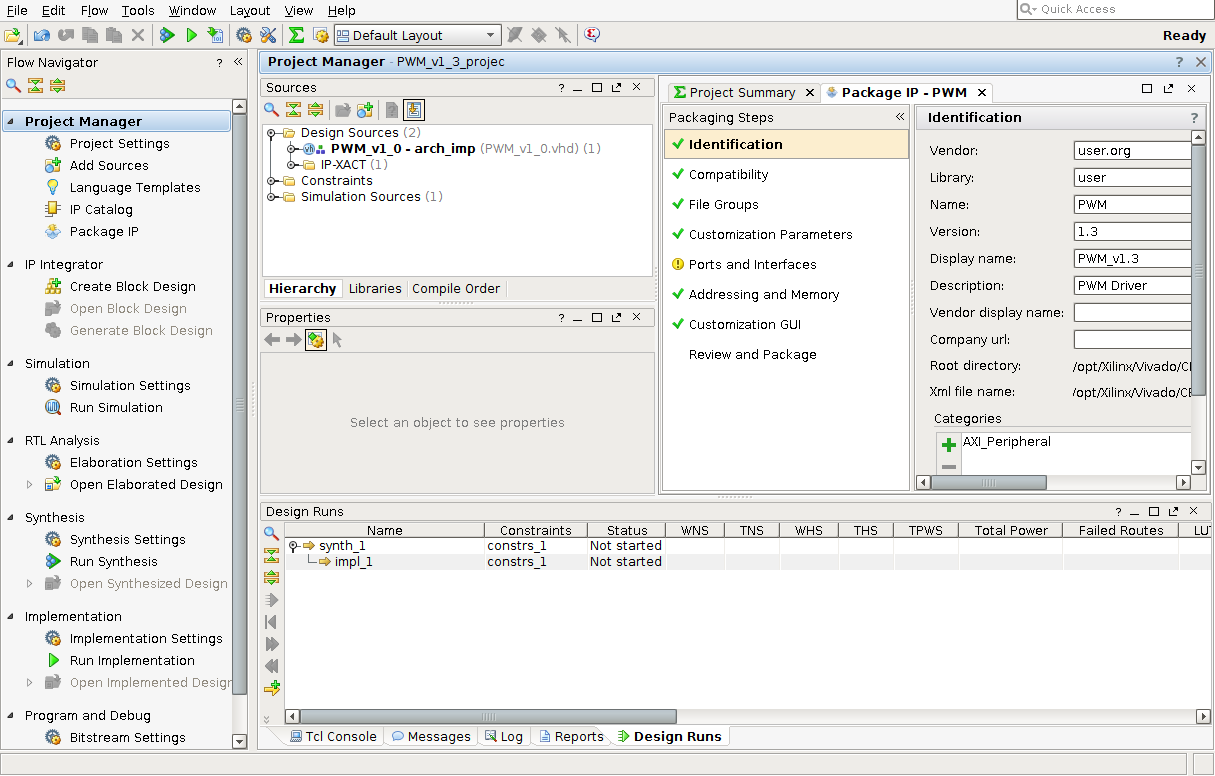
\includegraphics[width=0.85\textwidth]{img/ip.png}
    \caption{IP Project Structure}
    \label{fig:ip}
\end{figure}


\noindent\rule{16.5cm}{1pt}

\noindent\begin{minipage}{.1\textwidth}
  \centering
  
\includegraphics[height=1.5cm]{img/icon.png}
\end{minipage}
\begin{minipage}{.8\textwidth}
In this exercise, you will need to change the following parameter \textbf{PWM\_LEDs\_COUNTER\_PWM} to obtain a PWM frequency for the LEDs of 2kHz. Check its usage in this file and consider an input clock frequency of 50MHz.
\end{minipage}%

\noindent\rule{16.5cm}{1.5pt}

After modifying the frequency, you need to re-package the design. In order to do so, go back in the Package IP window and click on the Steps that are not checked green. Merge the changes and finally press the \textit{Review and Package} step and follow the indications from the window. Afterwards, the program will ask you if you want to exit. Press OK, and now you should be back in the previous project.

Now, the environment will detect a change in the IP and will ask you to update your component, as in Figure \ref{fig:upgrade_ip}. Press \textbf{Upgrade Selected}, check in the \textbf{Synthesis Option: Global} and now the changes should take place. 
Don't panic if you see the following error: {\color{red} ERROR: BD 41\-758 The following clock pins are not connected to a valid clock source: HP0\_ACLK}, we have not configured the Processing System yet. 

 
 \begin{figure}[h!]
    \centering
    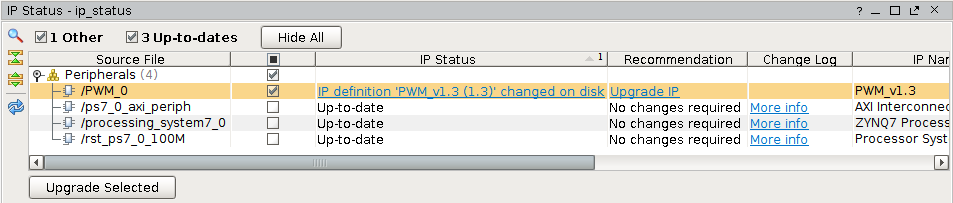
\includegraphics[width=0.85\textwidth]{img/upgrade.png}
    \caption{Upgrade IP Window}
    \label{fig:upgrade_ip}
\end{figure}




 \item Create PWM output ports
 
We need to create PWM outputs, in order to assign them to our board. Click on each PWM output and press CTRL-T or the Make External 
\includegraphics[width = 0.5cm]{img/make_exernal.png} symbol from the Menu. Do so for all the 4 ports. Now your IP should look like in Figure \ref{fig:pwm_logic_block}. You can also assign Highlight colors if you want.

 \item Configure the ZYNQ7 Processing System
 
Double click on the ZYNQ7 Processing System IP will open a user-friendly interface for selecting the clocks/memory/IOs. Now, you need to follow the next sub-steps:
\begin{itemize}
\item  \textbf{Zynq Block Diagram} 

Take some time to look at the diagram in order to understand the interface between PS and PL. Ask your tutor for further details, as this diagram is extremely important for future development with this board. 

\item \textbf{PS-PL Configuration}

This part will solve our previous error. We don't need high performance slave interface, so just deselect the \textit{S AXI HPO Interface}. Make sure everything is deselected as well.

\item \textbf{Peripherals I/O Pins}
Deselect everything apart from UART, as we want to transmit through serial interface(USB-UART) different messages from the board. Make sure both Bank 0 and Bank 1 is set to LVCMOS 3.3V. 

\noindent\rule{16.5cm}{1pt}

\noindent\begin{minipage}{.1\textwidth}
  \centering
  
\includegraphics[height=1.5cm]{img/icon.png}
\end{minipage}
\begin{minipage}{.8\textwidth}
Verify which UART (0 or 1) can be used in our case using the USB-UART cable. Look into the datasheet of the board: \url{http://www.myirtech.com/download/Zynq7000/Z-TURN_SCH_V4_20150326.pdf}
\end{minipage}%

\noindent\rule{16.5cm}{1pt}

\item \textbf{MIO Configuration}

If you did everything correctly in the previous step, now you should be able to see only UART selected.


\item \textbf{Clock Configuration}
Let everything as default, apart from \textbf{PL Fabric Clocks}. Roll the clocks down and deselect FCLK\_CLK1. As well, change the FCLK\_CLK0 to 50MHz.


\item \textbf{DDR Configuration}
Delect \textbf{Enable DDR}
\end{itemize}

Now press OK. Your ZYNQ7 Processing System should look more simplistic now, and easier to understand. 

\item Create VHDL Wrapper

From the block design, we need to create the VHDL code. Therefore, in the Project Sources - Design Sources, you need to right click on the \textbf{Peripherals Peripherals.bd} and select \textit {Create HDL Wrapper}. Let the default option and press OK. Now the VHDL Wrapper should have been created. Verify that the signals PWM\_RED, PWM\_BLUE, PWM\_GREEN and PWM\_BUZZER appear instantiated. 

 \item Create Constraint File
 
The Constraint File is used in the implementation phase. After the synthesis will be run, and the available top-level nets are thus "known", they will be thus matched to the "real" pins.
  
Right click on the Constraints directory and Add Source (Add or Create Constraints), then click finish, after you give the file a name.

Open it and write the following code that will define the nets and their dedicated ports.

\begin{minted}{vhdl}
## LED RED
set_property IOSTANDARD LVCMOS33 [get_ports PWM_RED]
set_property PACKAGE_PIN XX [get_ports PWM_RED]

## LED BLUE
set_property IOSTANDARD LVCMOS33 [get_ports PWM_BLUE]
set_property PACKAGE_PIN XX [get_ports PWM_BLUE]

## LED GREEN
set_property IOSTANDARD LVCMOS33 [get_ports PWM_GREEN]
set_property PACKAGE_PIN XX [get_ports PWM_GREEN]

## LED BUZZER
set_property IOSTANDARD LVCMOS33 [get_ports PWM_BUZZER]
set_property PACKAGE_PIN XX [get_ports PWM_BUZZER]

set_property CFGBVS VCCO [current_design]
set_property CONFIG_VOLTAGE 3.3 [current_design]

\end{minted}

\noindent\rule{16.5cm}{1pt}

\noindent\begin{minipage}{.1\textwidth}
  \centering
  
\includegraphics[height=1.5cm]{img/icon.png}
\end{minipage}
\begin{minipage}{.8\textwidth}
Open the next design file of the board and check Table 1-2 (page 5). Match the Default Function with our application and replace the XX with the specific pin (BGA column)
\url{http://www.myirtech.com/download/Zynq7000/Z-turnBoard.pdf}
\end{minipage}%

\noindent\rule{16.5cm}{1pt}


\item Generate the bitstream and export the hardware


Now, the project needs to be synthesized, implemented and finally the bitstream must 
be generated.
The bitstream is, as the name says, a binary sequence which indicates which connections inside the FPGA must be activated. That's why it is politically corect to call "configure an FPGA" and not "programme an FPGA".

To generate the bitstream, look into the Flow Manager on the left of the screen and press \textbf{Generate Bitstream (Figure \ref{fig:export_hardware_generate_bitstream})}. You will need to wait a bit longer until the bitstream is created. Check for errors in the process and solve them. Now, that the bitstream was successfully created, we need to export the hardware such as we can interact with it using the ARM dual-core microcontroller. 

To export the hardware, press \textbf{File $>$ Edit $>$ Export $>$ Export Hardware}. Tick \textit{Include bitstream} like in Figure \ref{fig:export_hardware_generate_bitstream}.


 \begin{figure}[h!]
\centering
\begin{minipage}{.425\textwidth}
  \centering
  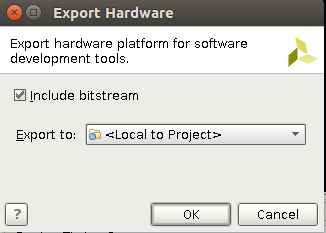
\includegraphics[width=0.8\linewidth]{img/export_hardware.png}
\end{minipage}%
\begin{minipage}{.425\textwidth}
  \centering
  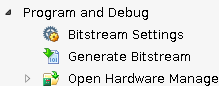
\includegraphics[width=0.8\linewidth]{img/generate_bitstream.png}
\end{minipage}
\caption{a) Export Hardware Window b) Generate Bitstream in Flow Manager}
\label{fig:export_hardware_generate_bitstream}
\end{figure}


\newpage
 \item Let's write some C code 

From now on, we will create the link between the fabric and the dual-core ARM microcontroller. For this, we will use \textbf{Xilinx Software Development Kit (XSDK)} which is the Integrated Design Environment for creating embedded applications. If you worked in Eclipse before, XSDK shall be a piece-of-cake, as it is build on the standard Eclipse IDE, with plugins and Xilinx-dedicated tools. 

To open it, press \textbf{File $>$ Launch SDK}. Now, the hardware shall be automatically imported in XSDK and now you can create a software application (Figure \ref{fig:sdk_first_page}).



 
 \begin{figure}[h!]
    \centering
    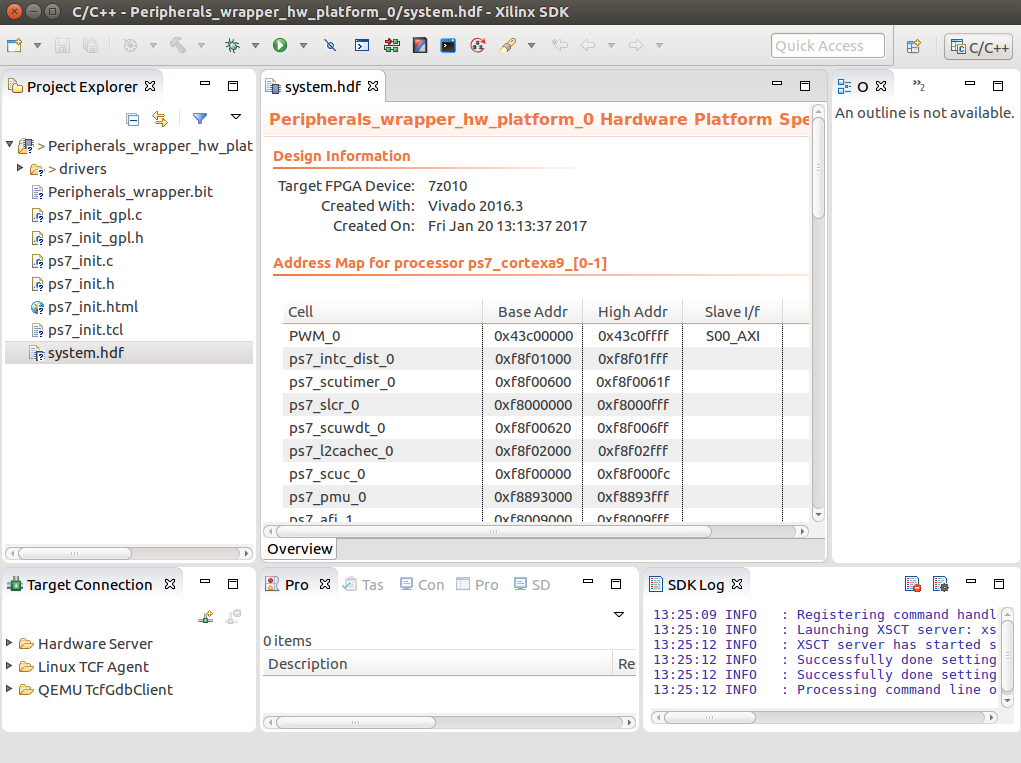
\includegraphics[width=0.85\textwidth]{img/xsdk_first_page.png}
    \caption{XSDK First Page after bitstream was exported}
    \label{fig:sdk_first_page}
\end{figure}



 \item Our first "Hello World Application"

Select \textbf{File $>$ New $>$ Application Project}.

The New Project dialog box opens. As Project Name, type the name desired, for example
\textit{LED\_Buzzer\_Controller}. Press \textbf{Next}. From the Available Templates, choose \textit{"Hello World"}. Click \textbf{Finish}. (Figure \ref{fig:start_proj_xsdk})


 \begin{figure}[h!]
\centering
\begin{minipage}{.425\textwidth}
  \centering
  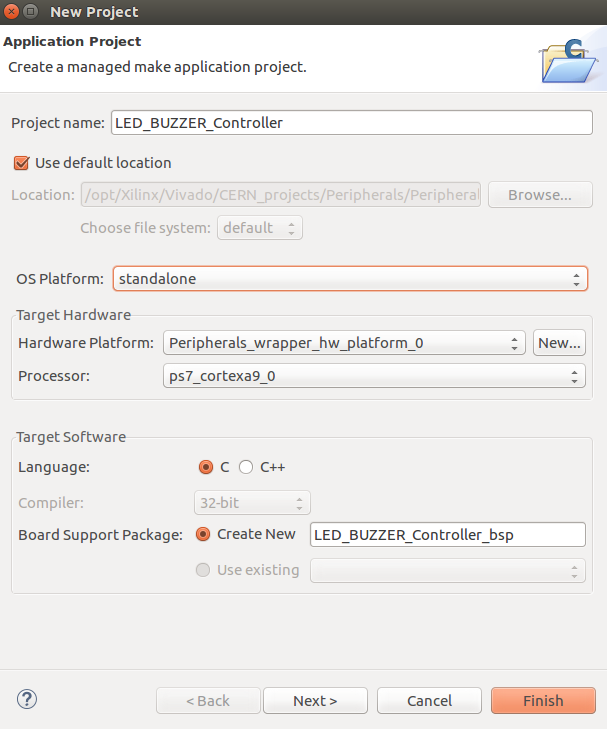
\includegraphics[width=0.8\linewidth]{img/app_project.png}
\end{minipage}%
\begin{minipage}{.425\textwidth}
  \centering
  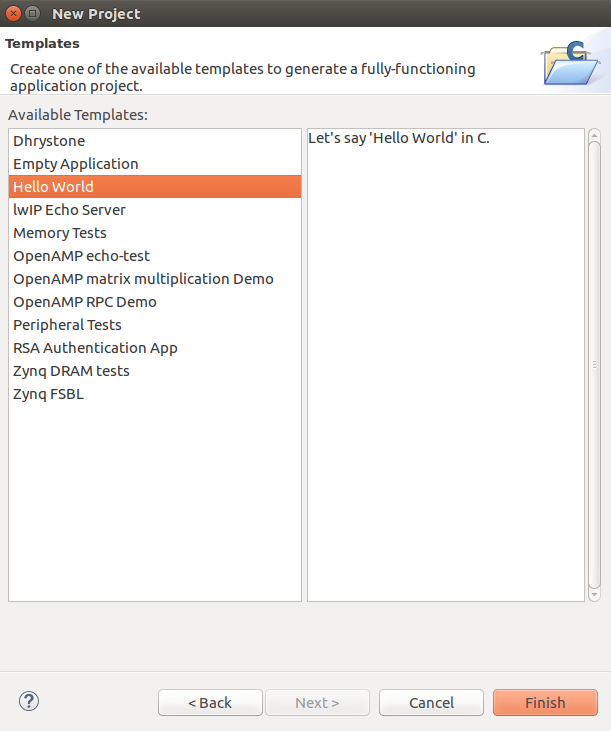
\includegraphics[width=0.8\linewidth]{img/hello_world.png}
\end{minipage}
\caption{Starting a project in XSDK}
\label{fig:start_proj_xsdk}
\end{figure}




\item Run the first application

To run the first application, you need to do the following simple steps:
\begin{myitemize}
\item Ensure that your board is powered on by connecting the Mini-USB to USB cable from computer to the USB\_UART mini-usb socket. This connectivity will also allow us transmit and receive data through serial communication.
\item 
\end{myitemize}

\end{enumerate}


















\clearpage

\section{LINUX OS on System on Chip}


\subsection{Introduction}

The current kit comes with Ubuntu 12.04 installed on a MicroSD card. Using this 
operating system, we will read the accelerometer data from the ADXL346 accelerometer
already mounted on board. This data will be feed into \textbf{bokeh}, which is a Python interactive visualization library which will also act as a server. In addition,
a control system will be added such as when the acceleration exceeds a certain treashold, a buzzer will start buzzering and an LED will turn red.

In real life, you can use this type of application to detect the high accelerations the astronauts are exposed during training and trigger a warning sound and light when certain threashold is exceeded.


\subsubsection{How is LINUX OS interacting with both the accelerometer and the buzzer?}

The I/O subsystem is the part of the Linux kernel that manages the various devices such as keyboards and mouse, devices usually used by any users. On top of this, it comes the Industrial I/O subsystem (IIO) that are analog to digital or digital to analog convertors, for example \textbf{the accelerometer, gyroscopes, proximity sensors} with the aim to extend the I/O subsystem. A typical device falling into the IIO category would be connected via SPI or I2C.




\subsubsection{How is LINUX OS interacting with the LEDs?}


\subsection{Let's get started!}

Now, we will move on with running an operating system on the System on Chip. For this, we will do the following steps:
\begin{myitemize}
\item you disconnected the JTAG cable used previously to programme the board
\item the mini SD Card is inserted in its socket
\item find Jumper 1 and Jumper 2 (JP1 and JP2) and make sure they are in the following order:
\begin{minted}{c}
JP1 OFF 
JP2 ON
\end{minted}
\end{myitemize}


When previously steps are done, you will see the RGB LED blinking on the board. It is very
important to make these configurations before moving on to the next section of the lab.

\subsection{Further configurations}

The SD card contains the image of Ubuntu 12.04 and will boot it on the board at every restart.

\subsubsection{Screen}

\subsubsection{File transfer between host computer and the board}

% Connect a screen to see that it works

% Open a terminal and communicate 

% Send a file through SSH

\subsection{Interact with the RGB LED and the Buzzer}




\subsection{Webserver}
Now, we will learn how to display the accelerometer values on an webserver running
on the host computer.



 %Each device provides one or more /dev/input/eventN nodes that a process can interact with. For example  reading events from the device.


 %The events themselves are in the form of struct input_event, defined in linux/input.h and consist of a event type (relative, absolute, key, ...) and an event code specific to the type (x axis, left button, etc.).

 %Any event coming from the physical hardware goes into the kernel's input subsystem and is converted to an evdev event that is then available on the event node.



\subsection{Booting LINUX with System on Chip}

\subsection{Interfacing the accelerometer + webserver}
 
 
%-------------------------------------------------------------------------------
% REFERENCES
%-------------------------------------------------------------------------------
\newpage
\section*{Reading List}
\addcontentsline{toc}{section}{Reading List}


  

\end{document}

%-------------------------------------------------------------------------------
% SNIPPETS
%-------------------------------------------------------------------------------

%\begin{figure}[!ht]
%	\centering
%	\includegraphics[width=0.8\textwidth]{file_name}
%	\caption{}
%	\centering
%	\label{label:file_name}
%\end{figure}

%\begin{figure}[!ht]
%	\centering
%	\includegraphics[width=0.8\textwidth]{graph}
%	\caption{Blood pressure ranges and associated level of hypertension (American Heart Association, 2013).}
%	\centering
%	\label{label:graph}
%\end{figure}

%\begin{wrapfigure}{r}{0.30\textwidth}
%	\vspace{-40pt}
%	\begin{center}
%		\includegraphics[width=0.29\textwidth]{file_name}
%	\end{center}
%	\vspace{-20pt}
%	\caption{}
%	\label{label:file_name}
%\end{wrapfigure}

%\begin{wrapfigure}{r}{0.45\textwidth}
%	\begin{center}
%		\includegraphics[width=0.29\textwidth]{manometer}
%	\end{center}
%	\caption{Aneroid sphygmomanometer with stethoscope (Medicalexpo, 2012).}
%	\label{label:manometer}
%\end{wrapfigure}

%\begin{table}[!ht]\footnotesize
%	\centering
%	\begin{tabular}{cccccc}
%	\toprule
%	\multicolumn{2}{c} {Pearson's correlation test} & \multicolumn{4}{c} {Independent t-test} \\
%	\midrule	
%	\multicolumn{2}{c} {Gender} & \multicolumn{2}{c} {Activity level} & \multicolumn{2}{c} {Gender} \\
%	\midrule
%	Males & Females & 1st level & 6th level & Males & Females \\
%	\midrule
%	\multicolumn{2}{c} {BMI vs. SP} & \multicolumn{2}{c} {Systolic pressure} & \multicolumn{2}{c} {Systolic Pressure} \\
%	\multicolumn{2}{c} {BMI vs. DP} & \multicolumn{2}{c} {Diastolic pressure} & \multicolumn{2}{c} {Diastolic pressure} \\
%	\multicolumn{2}{c} {BMI vs. MAP} & \multicolumn{2}{c} {MAP} & \multicolumn{2}{c} {MAP} \\
%	\multicolumn{2}{c} {W:H ratio vs. SP} & \multicolumn{2}{c} {BMI} & \multicolumn{2}{c} {BMI} \\
%	\multicolumn{2}{c} {W:H ratio vs. DP} & \multicolumn{2}{c} {W:H ratio} & \multicolumn{2}{c} {W:H ratio} \\
%	\multicolumn{2}{c} {W:H ratio vs. MAP} & \multicolumn{2}{c} {\% Body fat} & \multicolumn{2}{c} {\% Body fat} \\
%	\multicolumn{2}{c} {} & \multicolumn{2}{c} {Height} & \multicolumn{2}{c} {Height} \\
%	\multicolumn{2}{c} {} & \multicolumn{2}{c} {Weight} & \multicolumn{2}{c} {Weight} \\
%	\multicolumn{2}{c} {} & \multicolumn{2}{c} {Heart rate} & \multicolumn{2}{c} {Heart rate} \\
%	\bottomrule
%	\end{tabular}
%	\caption{Parameters that were analysed and related statistical test performed for current study. BMI - body mass index; SP - systolic pressure; DP - diastolic pressure; MAP - mean arterial pressure; W:H ratio - waist to hip ratio.}
%	\label{label:tests}
%\end{table}